\documentclass[12pt]{report}

\usepackage[left=0.75in, right=0.75in, top=0.75in, bottom=0.75in]{geometry}
\setlength\parindent{0pt}

\usepackage{graphicx, amsmath,anonchap,tabularx,multicol, array, color}

\usepackage{enumitem}
\setlist{noitemsep}
\setlist{nolistsep}

\begin{document}
\pagestyle{empty}

\textbf{Warm-up Instructions:} Whenever you see a new theorem, you should be sure to understand the hypotheses (requirements) of the theorem as well as the conclusions of the theorem. 

\bigskip
\textbf{\emph{\underline{The Mean Value Theorem (MVT)}}}: \\
\vspace{-1pt}
Suppose $y=f(x)$ is continuous on a closed interval $[a,b]$ and differentiable on the interval's interior $(a,b)$. Then there is at least one point $c$ in $(a,b)$ at which $\displaystyle\frac{f(b)-f(a)}{b-a}=f'(c)$
\vspace{1pt}
\begin{enumerate}
\item What are the requirements of the MVT? \\
\vspace{.1in}\\
We need \underline{\hspace{3in}} and \underline{\hspace{3in}} \\
\vspace{.1in}\\
Which of the graphs below satisfy the requirements of the MVT for the values of $a$ and $b$ indicated on the graphs? \\
\begin{multicols}{2}
	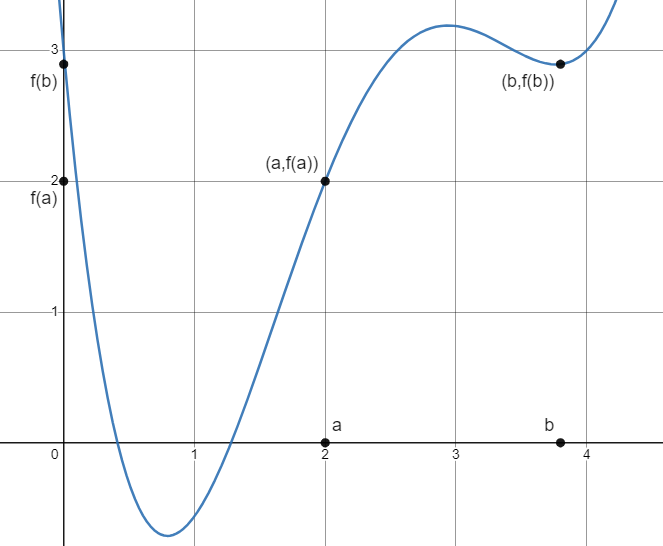
\includegraphics[scale=.5]{sat-mvt.PNG}
	
	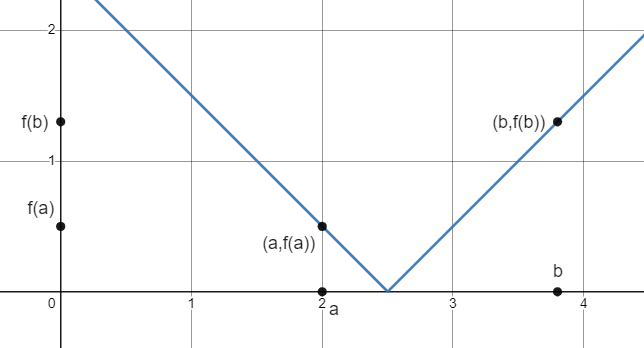
\includegraphics[scale=.5]{nosat-mvt.PNG}
\end{multicols}

\item What is the conclusion of the MVT? \\
\vspace{1in}\\
What does this mean? Can you interpret the conclusions using slope/AROC/IROC/Secant lines/Tangent lines in your explanation? Then sketch a picture of the meaning on the graphs above that meet the requirements.

\vspace{1.5 in}

%\item How do the ``rubber band functions" that we have handed out connect to the Mean Value Theorem? 
%can this become a desmos thing??
\end{enumerate}

\newpage
\iffalse
\begin{center}
\textbf{The Mean Value Theorem}
\end{center}

\textbf{Introduction:} \\

This section raises the question, ``Will the instantaneous rate of change at any point on an interval $[a, b]$ ever equal the average rate of change on the interval?" \\

It turns out that the answer is often yes, and the Mean Value Theorem tells us some situations in which the answer is yes.  \\

------------------------------------------------------------------------------------------------------------------------------------

\begin{center}
\textbf{The Mean Value Theorem (MVT)}
\end{center}

Suppose $y = f(x)$ is a function such that \\

\begin{enumerate}

\item $f$ is continuous on the closed interval $[a,b]$ \\

\item $f$ is differentiable on the interval's interior $(a,b)$.  \\

\end{enumerate}

Then there is \textit{at least one} point $c$ in $(a,b)$ at which \\

$$\frac{f(b) - f(a)}{b-a} = f'(c)$$

\begin{multicols}{2}

%\begin{figure}[h]
(From Thomas' Calculus) 

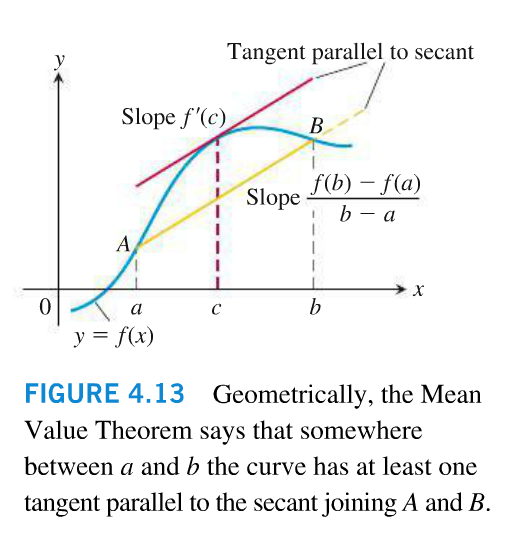
\includegraphics[scale=0.75]{MVTpic.png}

%\caption{A picture of a gull.}
%\end{figure}

\vspace{1in}
Interpretations of the difference quotient: \\

\begin{enumerate}

\item The slope of the secant line through the points $(a, f(a))$ and $(b, f(b))$. \\

\item The average (``mean") rate of change of $f(x)$ on the interval $[a,b]$. \\

\end{enumerate}

\end{multicols}

\newpage
\fi

\textbf{Examples:} \\

\textit{If the MVT is applicable (check first), find the value(s) of $c$ that satisfy the conclusion of the MVT.}  \\

\begin{enumerate}

\item $f(x) = x^2 + 2x -1, [0,1]$ \\

	\begin{enumerate}
	
	\item Continuous on $[a,b]?$
	
	\vspace{0.5 in}
	
	\item Differentiable on interior $(a,b)$? 
	
	\vspace{0.5 in}
	
	\item Find $c$ (If applicable): 
	
	\vspace{1 in}
	
	\end{enumerate}
	
\iffalse\item $g(x) = \sin(\frac{1}{x}), [-\pi,0]$ \\

\begin{enumerate}
	
	\item Continuous on $[a,b]?$
	
	\vspace{0.5 in}
	
	\item Differentiable on interior $(a,b)$? 
	
	\vspace{0.5 in}
	
	\item Find $c$ (If applicable): 
	
	\vspace{0.5 in}

\end{enumerate}
\fi

\item $h(x)$ on the indicated intervals (Note the hole):

\begin{multicols}{2}

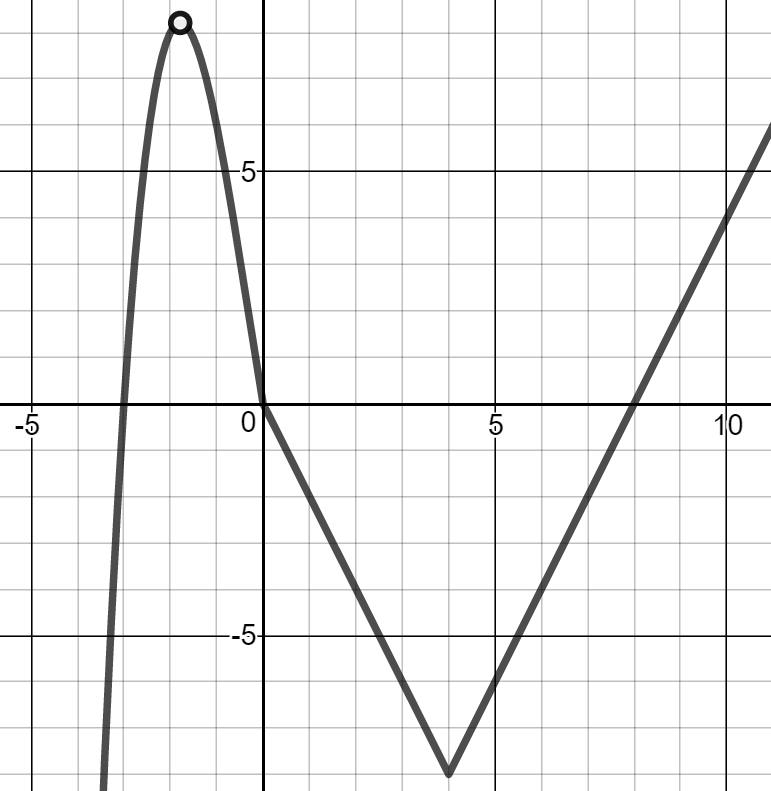
\includegraphics[scale=0.5]{MVTexample.png}

\begin{itemize}

\item[ ] \;\;\;(a)\;\;$[-2,0]$

\vspace{1.5 in}

\item[ ] \;\;\;(b)\;\;$[0,1]$


\end{itemize}

\end{multicols}



\item Fred enters a 60 mph highway at 7:30 with his friends Daphne, Velma, Shaggy and their dog Scooby. They stay on the highway for 20 miles and exit the highway at 7:45. They are immediately pulled over by the police.  Why did he get pulled over?  (Hint: Use the MVT - be sure to justify why you can use it!)

\end{enumerate}

\newpage
\begin{itemize}
	\item[4.] Create a counterexample for the following false statement: \\

\begin{center}
	Suppose $y=f(x)$ is continuous on $[a,b]$. Then there is at least one point $c$ in $(a,b)$ at which $\displaystyle{\frac{f(b)-f(a)}{b-a}=f'(c)}$.\\
\end{center}
Make sure your counter example includes all of the following:\\
\begin{itemize}
\item[(i)] A clearly defined function $f$ given graphically or with an equation and specific values for $a$ and $b$ (Hint: One of the previous graphs may work here). \\
\vspace{2in}
\item[(ii)] Justify how the given function $f$, and the values $a$ and $b$ satisfy the hypothesis. \\
\vspace{1in}
\item[(iii)] Explain how the conclusion is not satisfied: This means you must show that there are no points $c$ in $(a,b)$
 at which $\displaystyle{\frac{f(b)-f(a)}{b-a}=f'(c)}$.
\end{itemize}
\end{itemize}

\newpage
\textbf{Additional Examples and Explanations:} \\

\emph{\underline{Check Point}}: Find the value(s) of $c$ that satisfy the equation in the conclusion of the MVT for\\
$f(x)=e^{\frac{1}{3}x}$ on the interval $[0,3]$

\bigskip

\textcolor{blue}{Is $f(x)$ continuous on the interval $[0,3]$?} \textcolor{red}{Yes! ($f$ is continuous everywhere.)}

\textcolor{blue}{Is $f(x)$ differentiable on the interval $(1,3)$?} \textcolor{red}{Yes! $f'(x)=\displaystyle{\frac{1}{3}e^{\frac{1}{3}x}}$.}

\textcolor{blue}{Find $c$ in $(0,3)$:} 

\textcolor{red}{$$\frac{f(3)-f(0)}{3-0}=f'(c)$$}
\textcolor{red}{$$\frac{e^{1}-e^{0}}{3}=\displaystyle{\frac{1}{3}e^{\frac{1}{3}x}}$$}
\textcolor{red}{$$e-1=\displaystyle{e^{\frac{1}{3}x}}$$}
\textcolor{red}{$$\ln(e-1)=\ln\left(e^{\frac{1}{3}x}\right)$$}
\textcolor{red}{$$\ln(e-1)=\frac{1}{3}x\Rightarrow x=3\ln(e-1)\approx 1.624$$}

\bigskip

\emph{\underline{Check Point}}: Why might the MVT's conclusion be untrue if $f(x)$ were \textbf{not continuous} on $[a,b]$?

\textcolor{red}{Lots of possibilities here.  The key is that if you don't have the continuity on the closed interval and differentiability on the open interval, then you are not guaranteed the conclusion.}

\bigskip

\begin{multicols}{2}
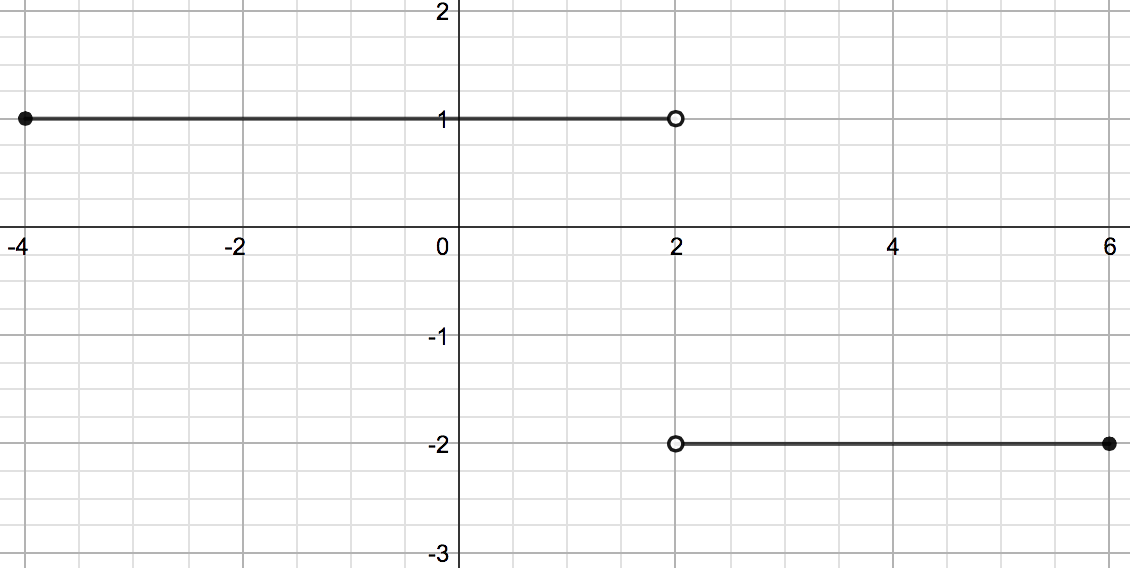
\includegraphics[scale=0.3]{MVT3.png}

\textcolor{red}{$\longleftarrow$ In this graph, the slope at all points (except at $x=2$) is 0, but the slope of the secant line connecting the endpoints is clearly negative.}
\end{multicols}

\bigskip

\begin{multicols}{2}
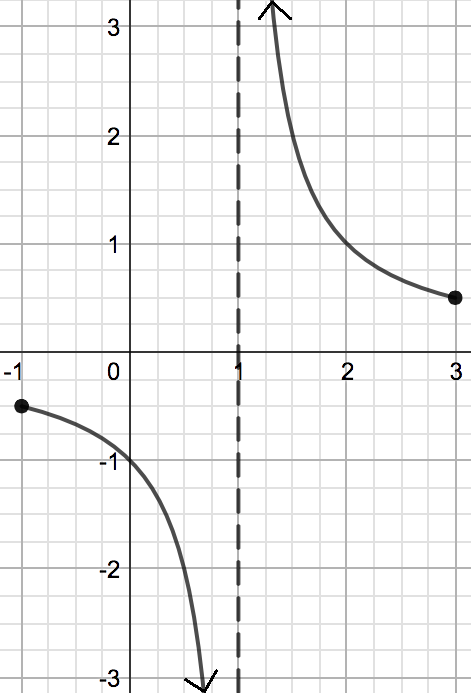
\includegraphics[scale=0.5]{MVT5edited.png}

\textcolor{red}{$\longleftarrow$ In this graph, the slope of the secant line connecting the endpoints is positive, but the slope at all points in between (except at $x=1$) is negative.}

\end{multicols}


\end{document}
